\documentclass[12pt]{exam}
\usepackage[brazil]{babel}
\usepackage{design_ASC}
\usepackage{enumitem}
\usepackage{subfig}
\usepackage{booktabs}

\setlength\parindent{0pt} %% Do not touch this
\newcolumntype{P}[1]{>{\arraybackslash}p{#1}}
\newcommand{\true}{V}
\newcommand{\false}{F}

%% -----------------------------
%% TITLE
%% -----------------------------
\title{Prova 2} %% Assignment Title

\author{Victor F. Ferrari\\ %% Student name
MO814A/MC937A - Tópicos in Computação Gráfica\\ %% Code and course name
\textsc{Universidade Estadual de Campinas}
}

\date{\today} %% Change "\today" by another date manually
%% -----------------------------
%% -----------------------------

%% %%%%%%%%%%%%%%%%%%%%%%%%%
\begin{document}
\setlength{\droptitle}{-5em}    
%% %%%%%%%%%%%%%%%%%%%%%%%%%
\maketitle

% --------------------------
% Start here
% --------------------------

% %%%%%%%%%%%%%%%%%%%
\section*{Questão 1}
% %%%%%%%%%%%%%%%%%%%
{\bfseries Correspondência. Para cada um dos seguintes conceitos, escreva o número do fragmento de sentença que completa corretamente a afirmação. Nenhuma explicação é necessária. A correspondência é uma-a-uma.}

\begin{enumerate}[label=\alph*)]
    \item Interseção raio-esfera... [\textbf{\ref{squared}}]
    \item Interseção raio-triângulo... [\textbf{\ref{lin}}]
    \item Um renderizador de ray tracing... [\textbf{\ref{pixels}}]
    \item Um \textit{fragment shader}... [\textbf{\ref{after}}]
    \item Um \textit{vertex shader}... [\textbf{\ref{before}}]
    \item Um renderizador de rasterização... [\textbf{\ref{obj}}]
    \item Uma B-spline cúbica... [\textbf{\ref{cont}}]
    \item Uma spline Hermite... [\textbf{\ref{tang}}]
\end{enumerate}

\begin{enumerate}
    \item ...envolve resolver um sistema linear 3x3. \label{lin}
    \item ...processa objetos um de cada vez. \label{obj}
    \item ...é executado antes da rasterização. \label{before}
    \item ...é executado após a rasterização. \label{after}
    \item ...envolve resolver uma equação quadrática. \label{squared}
    \item ...mantém a continuidade $C^2$ entre os segmentos. \label{cont}
    \item ...é definido a partir das posições e tangentes em seus pontos finais. \label{tang}
    \item ...processa pixels, um de cada vez. \label{pixels}
\end{enumerate}

% %%%%%%%%%%%%%%%%%%%
\section*{Questão 2}
% %%%%%%%%%%%%%%%%%%%
{\bfseries Verdadeiro ou Falso.}

\begin{enumerate}[label=\alph*)]
    \item Em um algoritmo de \textit{ray tracing}, o loop externo é sobre pixels e o loop interno é sobre objetos. (\true)
    \item Em um algoritmo de rasterização, o loop externo é sobre pixels e o loop interno é sobre objetos. (\false)
    \item Na rasterização, cada fragmento corresponde exatamente a um pixel. (\true)
    \item Na rasterização, cada pixel corresponde exatamente a um fragmento. (\false)
    \item No modelo Blinn-Phong, o destaque especular aumenta de tamanho à medida que o expoente aumenta. (\false)
    \item No modelo Blinn-Phong, o ponto mais brilhante do destaque especular aumenta de brilho à medida que o destaque fica menor. (\true)
    \item As transformações de perspectiva preservam as linhas retas. (\true)
    \item Transformações afins preservam linhas paralelas. (\true)
    \item As transformações de perspectiva preservam linhas paralelas. (\false)
    \item As transformações do corpo rígido 3D são comutadas. (\false)
\end{enumerate}

% %%%%%%%%%%%%%%%%%%%
\section*{Questão 3}
% %%%%%%%%%%%%%%%%%%%
{\bfseries \textit{Shading}. Diga 3 diferenças entre \textit{Flat shading}, \textit{Gouraud shading}, e \textit{Phong shading}.}

\begin{table}[tbh]
    \centering
    \scalebox{1.25}{%
    \scriptsize
    \begin{tabular}{@{}P{0.03\textwidth}|P{0.19\textwidth}|P{0.25\textwidth}|P{0.25\textwidth}@{}}
        \toprule
      \textbf{Dif.} & 
        \textit{Flat Shading} &
            \textit{Gouraud Shading}&
                \textit{Phong Shading}\\
      \midrule
      1 & 
        Usa uma normal por polígono. & 
            Usa uma normal por vértice. & 
                Usa uma normal por pixel, interpolada a partir dos vértices. \\
    \hline
      2& 
        É um método de execução muito rápida. & 
            É um método de execução razoavelmente rápida. & 
                É um método de execução lenta. \\
    \hline
      3& 
        É um método pouco realista e pouco preciso, que gera seções descontínuas entre os polígonos. & 
            É um método um pouco mais realista, mas ainda não é tão preciso como o ideal, e elimina a componente especular da luz.& 
                É um método bem mais realista e preciso, admite componente especular e é difícil de diferenciar modelos com poucos e muitos polígonos. \\
        \bottomrule
    \end{tabular}
    }
\end{table}

% %%%%%%%%%%%%%%%%%%%
\section*{Questão 4}
% %%%%%%%%%%%%%%%%%%%
{\bfseries \textit{Shading}. Qual dos 3 (\textit{flat shading}, \textit{Gouraud shading}, e \textit{Phong shading}) é o mais realista, especialmente para superfícies altamente curvas?.}

O modelo mais realista é o \textbf{Phong Shading}, especialmente para superfícies curvas. Isso se dá pois, nele, a equação de iluminação é solucionada para cada pixel. Por isso, em superfícies curvas, nas quais a solução dessa equação para um ponto interior do objeto pode ser bem diferente da solução no vértice, Phong shading fornece um resultado mais realista que os outros. Outros aspectos como os ângulos em relação ao observador e à fonte de luz também afetam a solução da equação, e isso é muito variável no interior de superfícies curvas.

% %%%%%%%%%%%%%%%%%%%
\section*{Questão 5}
% %%%%%%%%%%%%%%%%%%%
{\bfseries \textit{Shader}. Qual shader é executado primeiro no pipeline gráfico: \textit{vertex} ou \textit{fragment}?}

O \textbf{vertex shader} é executado primeiro no pipeline. Ele é executado sobre os vértices geométricos, enquanto o fragment shader é executado após a rasterização.

% %%%%%%%%%%%%%%%%%%%
\section*{Questão 6}
% %%%%%%%%%%%%%%%%%%%
{\bfseries \textit{Shader}. Que tipo de variável do \textit{vertex shader} tem o mesmo valor para todos os vértices? [Selecionar uma opção]}

\begin{enumerate}[label=\alph*)]
    \item \textbf{\textit{uniform variable}.}
    \item \textit{varying variable}.
    \item \textit{constant variable}.
    \item \textit{variable constant}.
    \item \textit{lighting variable}.
\end{enumerate}

\textbf{Resposta: a)}

% %%%%%%%%%%%%%%%%%%%
\section*{Questão 7}
% %%%%%%%%%%%%%%%%%%%
{\bfseries \textit{Shader}. No GLSL, o que é swizzling?}

\textit{Swizzling} é a opção presente no GLSL de manipular arrays não apenas pelas suas posições, mas pelo nome de seus componentes. Isso permite a utilização de máscaras para mudar diversos componentes em uma única operação.

Exemplo: se um array C tem 4 posições, de nomes $r,g,b,a$, é possível usar a máscara C.gb para modificar as posições g e b diretamente, com apenas uma operação.

% %%%%%%%%%%%%%%%%%%%
\section*{Questão 8}
% %%%%%%%%%%%%%%%%%%%
{\bfseries \textit{Pipeline Gráfico}. Onde no pipeline gráfico ocorre o \textit{texture mapping}?}

O \textit{texture mapping} ocorre no \textbf{fragment shader}, ou seja, após a rasterização, durante o processamento dos fragmentos.

% %%%%%%%%%%%%%%%%%%%
\section*{Questão 9}
% %%%%%%%%%%%%%%%%%%%
{\bfseries \textit{Antialiasing}:}

\begin{enumerate}[label=\alph*)]
    \item Por que o \textit{aliasing} é um problema?
    
    \textit{Aliasing} é um problema pois gera artefatos na imagem que prejudicam a clareza do que quer ser demonstrado, e que podem ser desconfortáveis ao olho, como bordas serrilhadas, padrões falsos de texturas, etc. Em alguns casos esses artefatos são muito visíveis e atrapalham a constituição da cena.
    
    \item Quando surge o \textit{aliasing}?
    
    O \textit{aliasing} surge a partir de uma grande diferença entre a "frequência" necessária de medição, e a de medição. Ou seja, quando a imagem gerada não consegue capturar o formato correto da geometria. Isso ocorre, por exemplo, quando a imagem não tem resolução adequada para representar corretamente a figura, obtida por \textit{point sampling}.
    
    \item Descreva um método de \textit{antialiasing}.
    
    Um dos clássicos métodos de \textit{antialiasing} é a filtragem de "caixa" por \textit{supersampling}, que consiste em dividir um pixel em uma matriz quadrada (de, por exemplo, 5x5 elementos) e atribuir a ele intensidade correspondente à média da intensidade dos subpixels da matriz.
    
    \item Suponha que estamos renderizando um segmento de linha preta em um fundo branco em uma imagem em escala de cinza $6\times6$ com $1/\sqrt{2}$ pixels de espessura e vai das coordenadas de pixel (1, 1) a (4, 4), conforme ilustrado abaixo. A linha tem intensidade 0 e o fundo tem intensidade 1. Como seria o resultado usando seu método?.
    
    Inicialmente, dividimos os pixels que contém o segmento em uma matriz de 5x5 elementos. Em seguida, tiramos a média das intensidades dos subpixels da matriz, e aplicamos ao pixel original.
    
    \begin{figure}[H]
        \centering
        \subfloat[Original]{
        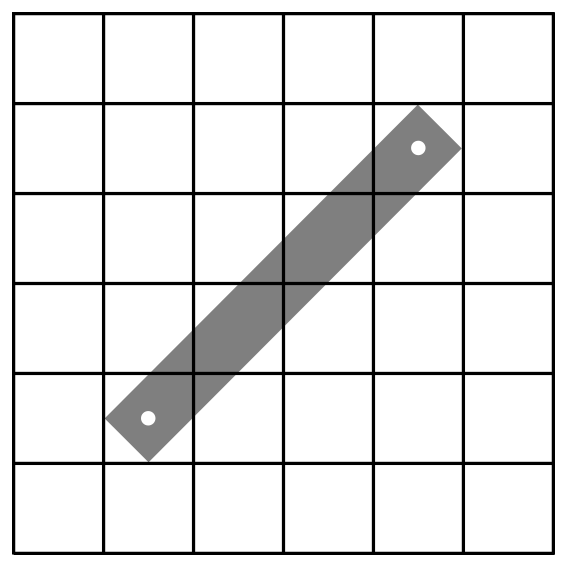
\includegraphics[width=0.4\textwidth]{images/11_orig.png}
        }
        \subfloat[Supersampling]{
        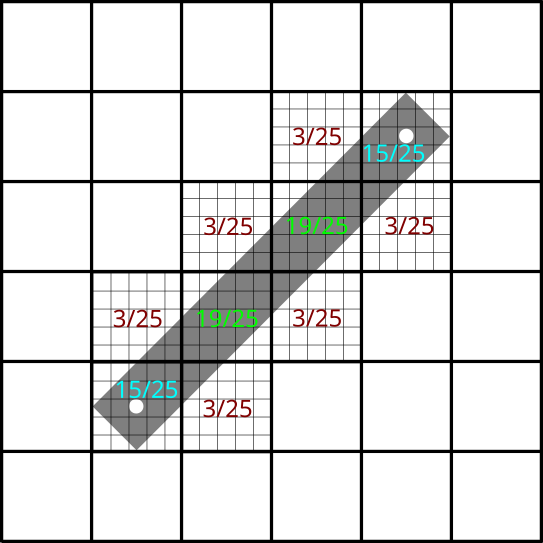
\includegraphics[width=0.4\textwidth]{images/11_super.png}
        }
        \qquad
        \subfloat[Resultado]{
        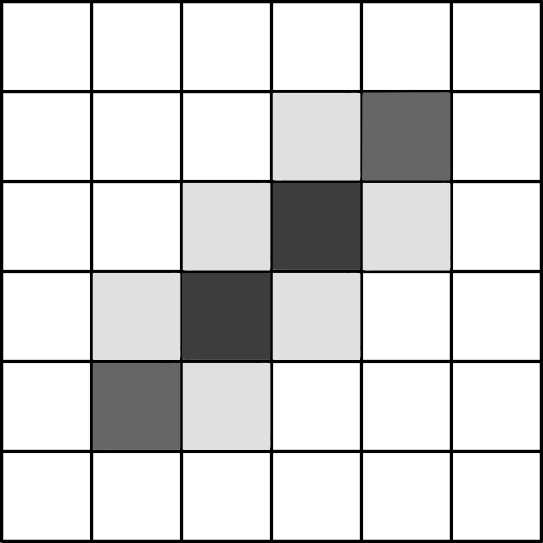
\includegraphics[width=0.4\textwidth]{images/11_final.png}
        }
        \caption{\textit{Box Filtering Antialiasing}}
        \label{fig:11}
    \end{figure}

\end{enumerate}

% %%%%%%%%%%%%%%%%%%%
\section*{Questão 10}
% %%%%%%%%%%%%%%%%%%%
{\bfseries Animação. Dê uma vantagem e uma desvantagem do uso da captura de movimento (\textit{motion capture}) para criar animação.}

Uma vantagem de captura de movimento é que, como a origem dos dados do movimento é uma gravação de movimentos reais, essa estratégia fornece dados bem realistas (se os dados forem bem capturados, como é comum atualmente) e imediatos, em grande quantidade.

Por outro lado, uma desvantagem do modo de animação é a dificuldade de edição e modificação desses dados, ou seja, a animação fica "presa" ao que foi gravado, além de estar "preso" a movimentos reais (movimentos que não respeitam leis da física não podem ser capturados).

% %%%%%%%%%%%%%%%%%%%
\section*{Questão 11}
% %%%%%%%%%%%%%%%%%%%
{\bfseries Animação. Suponha que desejemos animar uma bola quicando. Recebemos quadros-chave (\textit{keyframes}) para o movimento da bola. Os quadros-chave (\textit{keyframes}) estão amostrados nos tempos $T = 0, 1, 2, 3, 4, 5, 6$ com valores de altura associados de $H = 0, 5, 8, 9, 8, 5, 0$.}

\begin{enumerate}[label=\alph*)]
    \item Plote o gráfico de altura versus tempo usando interpolação linear entre os quadros-chave (\textit{keyframes}).
    
    Os pontos são interpolados em pares, por meio de funções lineares, resultando na seguinte imagem.
    
    \begin{figure}[ht]
        \centering
        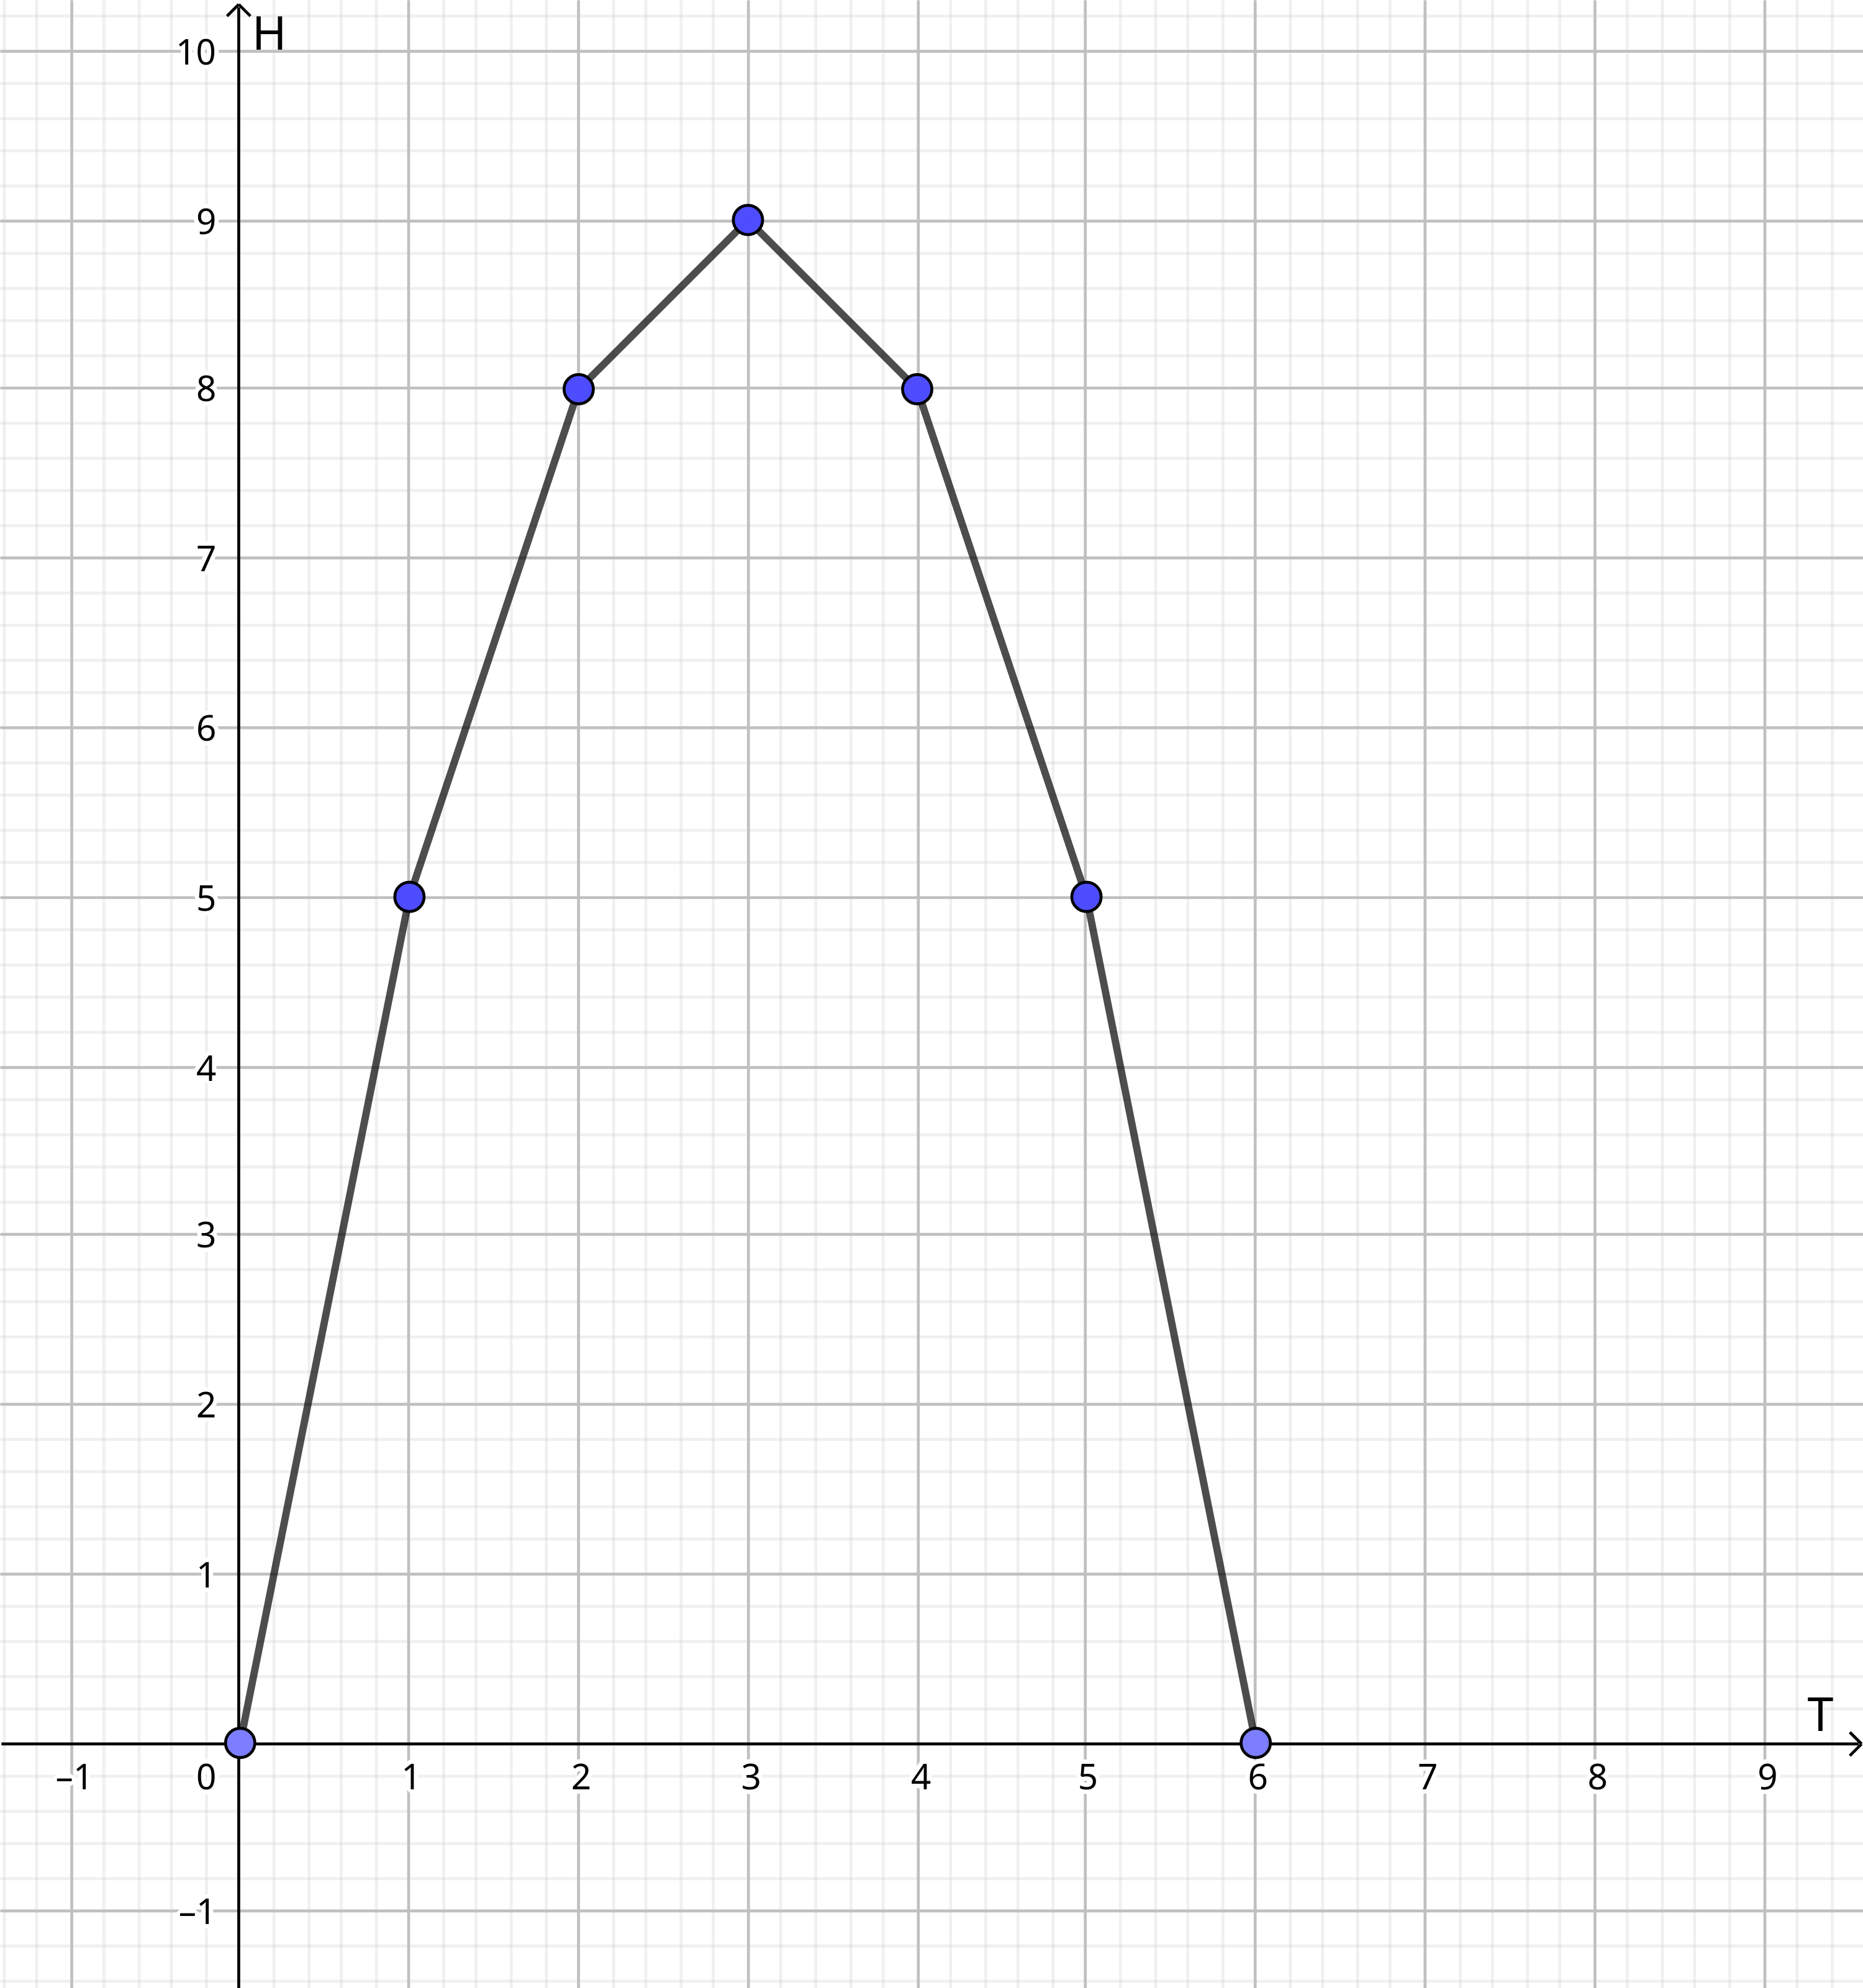
\includegraphics[width=0.5\textwidth]{images/fit.png}
        \caption{Gráfico Altura X Tempo}
        \label{fig:11a}
    \end{figure}
    
    \item Dê uma equação para a altura h(t) ao longo do intervalo t = 4 ... 5 usando interpolação linear.
    
    Considerando apenas o intervalo [4,5], uma equação entre esses 2 pontos seria a reta $H = -3T+20$.
\end{enumerate}

% %%%%%%%%%%%%%%%%%%%
\section*{Questão 12}
% %%%%%%%%%%%%%%%%%%%
{\bfseries Animação. Nuvens e multidões são exemplos de que tipo de sistema?}

É possível modelar nuvens e multidões como sistemas de \textbf{partículas}.

% %%%%%%%%%%%%%%%%%%%
\section*{Questão 13}
% %%%%%%%%%%%%%%%%%%%
{\bfseries Modelagem geométrica. Quais são algumas das razões pelas quais preferimos triângulos a outros tipos de polígonos?}

Triângulos são bons candidatos para primitivas pois todos os polígonos são trianguláveis, então é possível representar qualquer figura poligonal por meio de triângulos, e essa triangulação pode ser feita por algoritmos eficientes. Triângulos são também polígonos com poucos vértices, convexos e com poucas diferenças entre si. Por isso, há \textit{hardware} especializado para triângulos, o que incentiva ainda mais o uso.

% %%%%%%%%%%%%%%%%%%%
\section*{Questão 14}
% %%%%%%%%%%%%%%%%%%%
{\bfseries Iluminação. Quais são as diferentes classes de luzes que consideramos em computação gráfica? Quais são alguns exemplos do mundo real dos diferentes tipos?}

Os três tipos de reflexões do modelo de iluminação de Phong são \textbf{ambiente}, \textbf{difusa} e \textbf{especular}. Os tipos de luz do resultado de cada reflexão têm o mesmo nome. A luz ambiente é uma luz uniforme que é a união das reflexões secundárias de todos os objetos da cena, representando iluminação \textbf{indireta}. A luz difusa é refletida igualmente a todos os lados ao atingir um objeto. A luz especular é uma reflexão quase perfeita, refletindo exatamente a cena naquela direção se ideal, e causando um brilho caso contrário. Exemplos no mundo real estão a seguir.

\begin{itemize}
    \item Ambiente: poucos exemplos existem, pois é uma abstração. Algo próximo é um dia nublado, com pouca direcionalidade na iluminação, sendo mais uniforme.
    \item Difusa: luz refletida de giz ou outros materiais foscos.
    \item Especular Ideal: Espelho.
    \item Especular Não-Ideal: Objetos brilhantes como uma esfera de aço ou madeira polida.
\end{itemize}

% %%%%%%%%%%%%%%%%%%%
\section*{Questão 15}
% %%%%%%%%%%%%%%%%%%%
{\bfseries Iluminação. Difusa e Especular. Na figura 2D abaixo, temos o olho localizado à esquerda, um plano/linha ao longo da parte inferior e uma fonte de luz pontual para a direita; a luz está duas vezes mais distante do plano/linha do que o olho está. Os locais marcados e rotulados no plano/linha indicam o ponto mais próximo do olho e da luz. Para os fins desta pergunta, o ponto na frente do olho é usado como ponto do olho e a intensidade da luz NÃO atenua com a distância.}

\begin{enumerate}[label=\alph*)]
    \item Suponha que o plano/linha tenha apenas um componente de material difuso. Marque com um ’D’ na figura, em que o plano/linha aparecerá mais brilhante para o espectador.
    \item Suponha que o plano/linha tenha apenas um componente de material especular. Marque com um ’S’ na figura em que o plano/linha aparecerá mais brilhante para o espectador.
\end{enumerate}

\begin{figure}[ht]
    \centering
    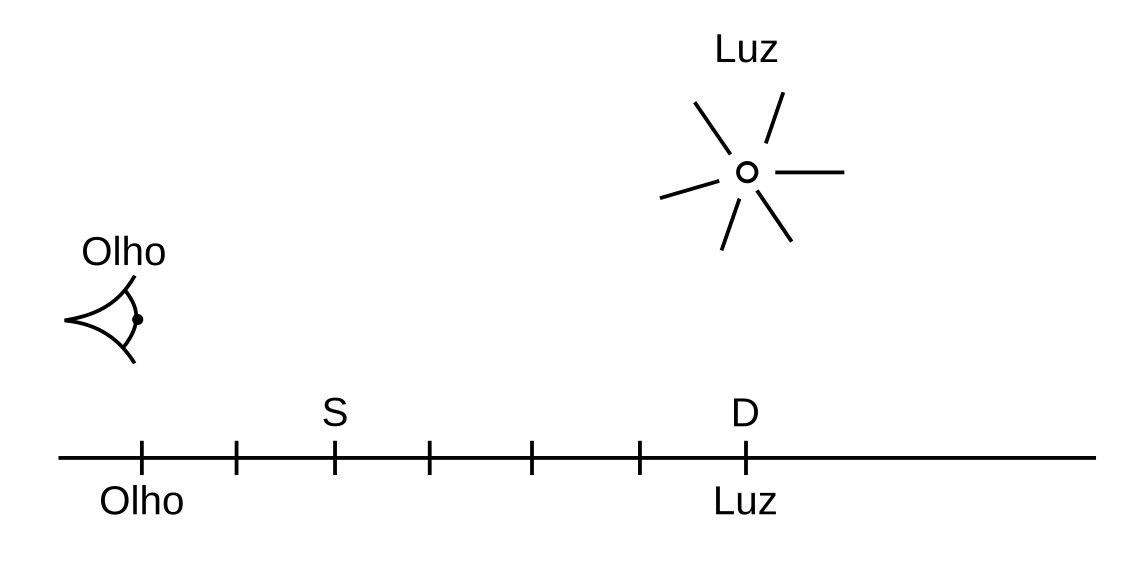
\includegraphics[width=0.8\textwidth]{images/15.jpg}
    \caption{Linha, luz e olho.}
    \label{fig:15}
\end{figure}

\textbf{a)}

Como, na equação de Phong, a luz difusa é dada pelo termo $I = Ck_d \cos{\theta}$, C é propriedade da luz, e $k_d$ é propriedade da superfície, temos que I é máximo quando $\cos{\theta}$ é máximo, ou seja, quando os vetores L e N são coincidentes. Isso ocorre no local onde a luz incide perpendicularmente sobre a superfície, ou seja, no ponto mais próximo à luz.

\textbf{b)}

Como, na equação de Phong, a luz especular é dada pelo termo $I = Ck_s \cos^n(\alpha)$, C é propriedade da luz, e $k_s$ é propriedade da superfície, temos que I é máximo quando $\cos{\alpha}$ é máximo, ou seja, quando os vetores R e E são coincidentes. Isso ocorre no local onde o ângulo da luz com a superfície é o mesmo que o ângulo do observador com a superfície.

Como a luz está com o dobro da distância perpendicular à superfície que o observador, a distância horizontal também deve ser o dobro, assim o ponto de maior brilho está a 2 unidades de distância horizontal do olho e 4 unidades de distância horizontal da luz.

% %%%%%%%%%%%%%%%%%%%
\section*{Questão 16}
% %%%%%%%%%%%%%%%%%%%
{\bfseries Iluminação. Uma importante técnica de renderização foi inventada ao pensar como a luz do sol brilha através de uma janela e se move para iluminar as paredes, o teto e o chão de uma sala. Indique essa técnica.}

Essa técnica é chamada de \textbf{radiosity}, importante técnica de iluminação global.

% %%%%%%%%%%%%%%%%%%%
\section*{Questão 17}
% %%%%%%%%%%%%%%%%%%%
{\bfseries Mapping. O que é \textit{bump mapping}? O que é \textit{displacement mapping}? Como eles diferem?}

\textit{Bump mapping} e \textit{displacement mapping} são técnicas de texturização usadas para representar detalhes. \textit{Bump mapping} é uma técnica que interpreta pixels da textura como normais, fazendo com que a imagem pareça mais complicada que a geometria é. \textit{Displacement mapping}, por outro lado, faz um deslocamento da geometria para adicionar mais detalhes.

A diferença entre as técnicas está no fato de que DM realmente altera a geometria, a posição da superfície na direção da normal, enquanto BM não modifica a geometria, apenas sua percepção. Por isso, DM é mais caro em termos de desempenho que BM.

% %%%%%%%%%%%%%%%%%%%
\section*{Questão 18}
% %%%%%%%%%%%%%%%%%%%
{\bfseries Hidden Surface Removal. Qual das alternativas a seguir não é um algoritmo de remoção de superfícies ocultas (\textit{hidden surface removal})? [Selecionar uma opção]}

\begin{enumerate}[label=\alph*)]
    \item Depth Sort
    \item Painter's Algorithm
    \item Z-Buffer
    \item \textbf{Nenhum Desses}
\end{enumerate}

\textbf{Resposta: d)}

% %%%%%%%%%%%%%%%%%%%
\section*{Questão 19}
% %%%%%%%%%%%%%%%%%%%
{\bfseries Textura. Indique a técnica de CG que pega um mapa de textura e cria uma hierarquia de versões em diferentes resoluções.}

Essa técnica de texturização é chamada de \textbf{mipmapping}.

% %%%%%%%%%%%%%%%%%%%
\section*{Questão 20}
% %%%%%%%%%%%%%%%%%%%
{\bfseries \textit{Bounding volume hierarchy}. Desenhe uma \textit{axis-aligned bounding box hierarchy} 2D para o seguinte conjunto de pontos, usando a estratégia \textit{topdown} usando divisão por mediana. O eixo mais largo deve ser dividido a cada vez. Os nós das folhas devem conter até dois (2) pontos cada. As linhas desenhadas não precisam ser perfeitas; eles serão tratados como estando na linha de grade mais próxima. Quatro cópias do mesmo diagrama foram fornecidas. Você só precisa completar um; se uma cópia ficar ilegível como resultado de correções, usar outra.}

Alguns pontos foram movidos de uma linha da grade para o interior de uma célula apenas por visualização, para indicar pertencimento a uma seção do plano. Como linhas passariam por cima deles, o resultado ficaria ambíguo.

\begin{figure}[ht]
    \centering
    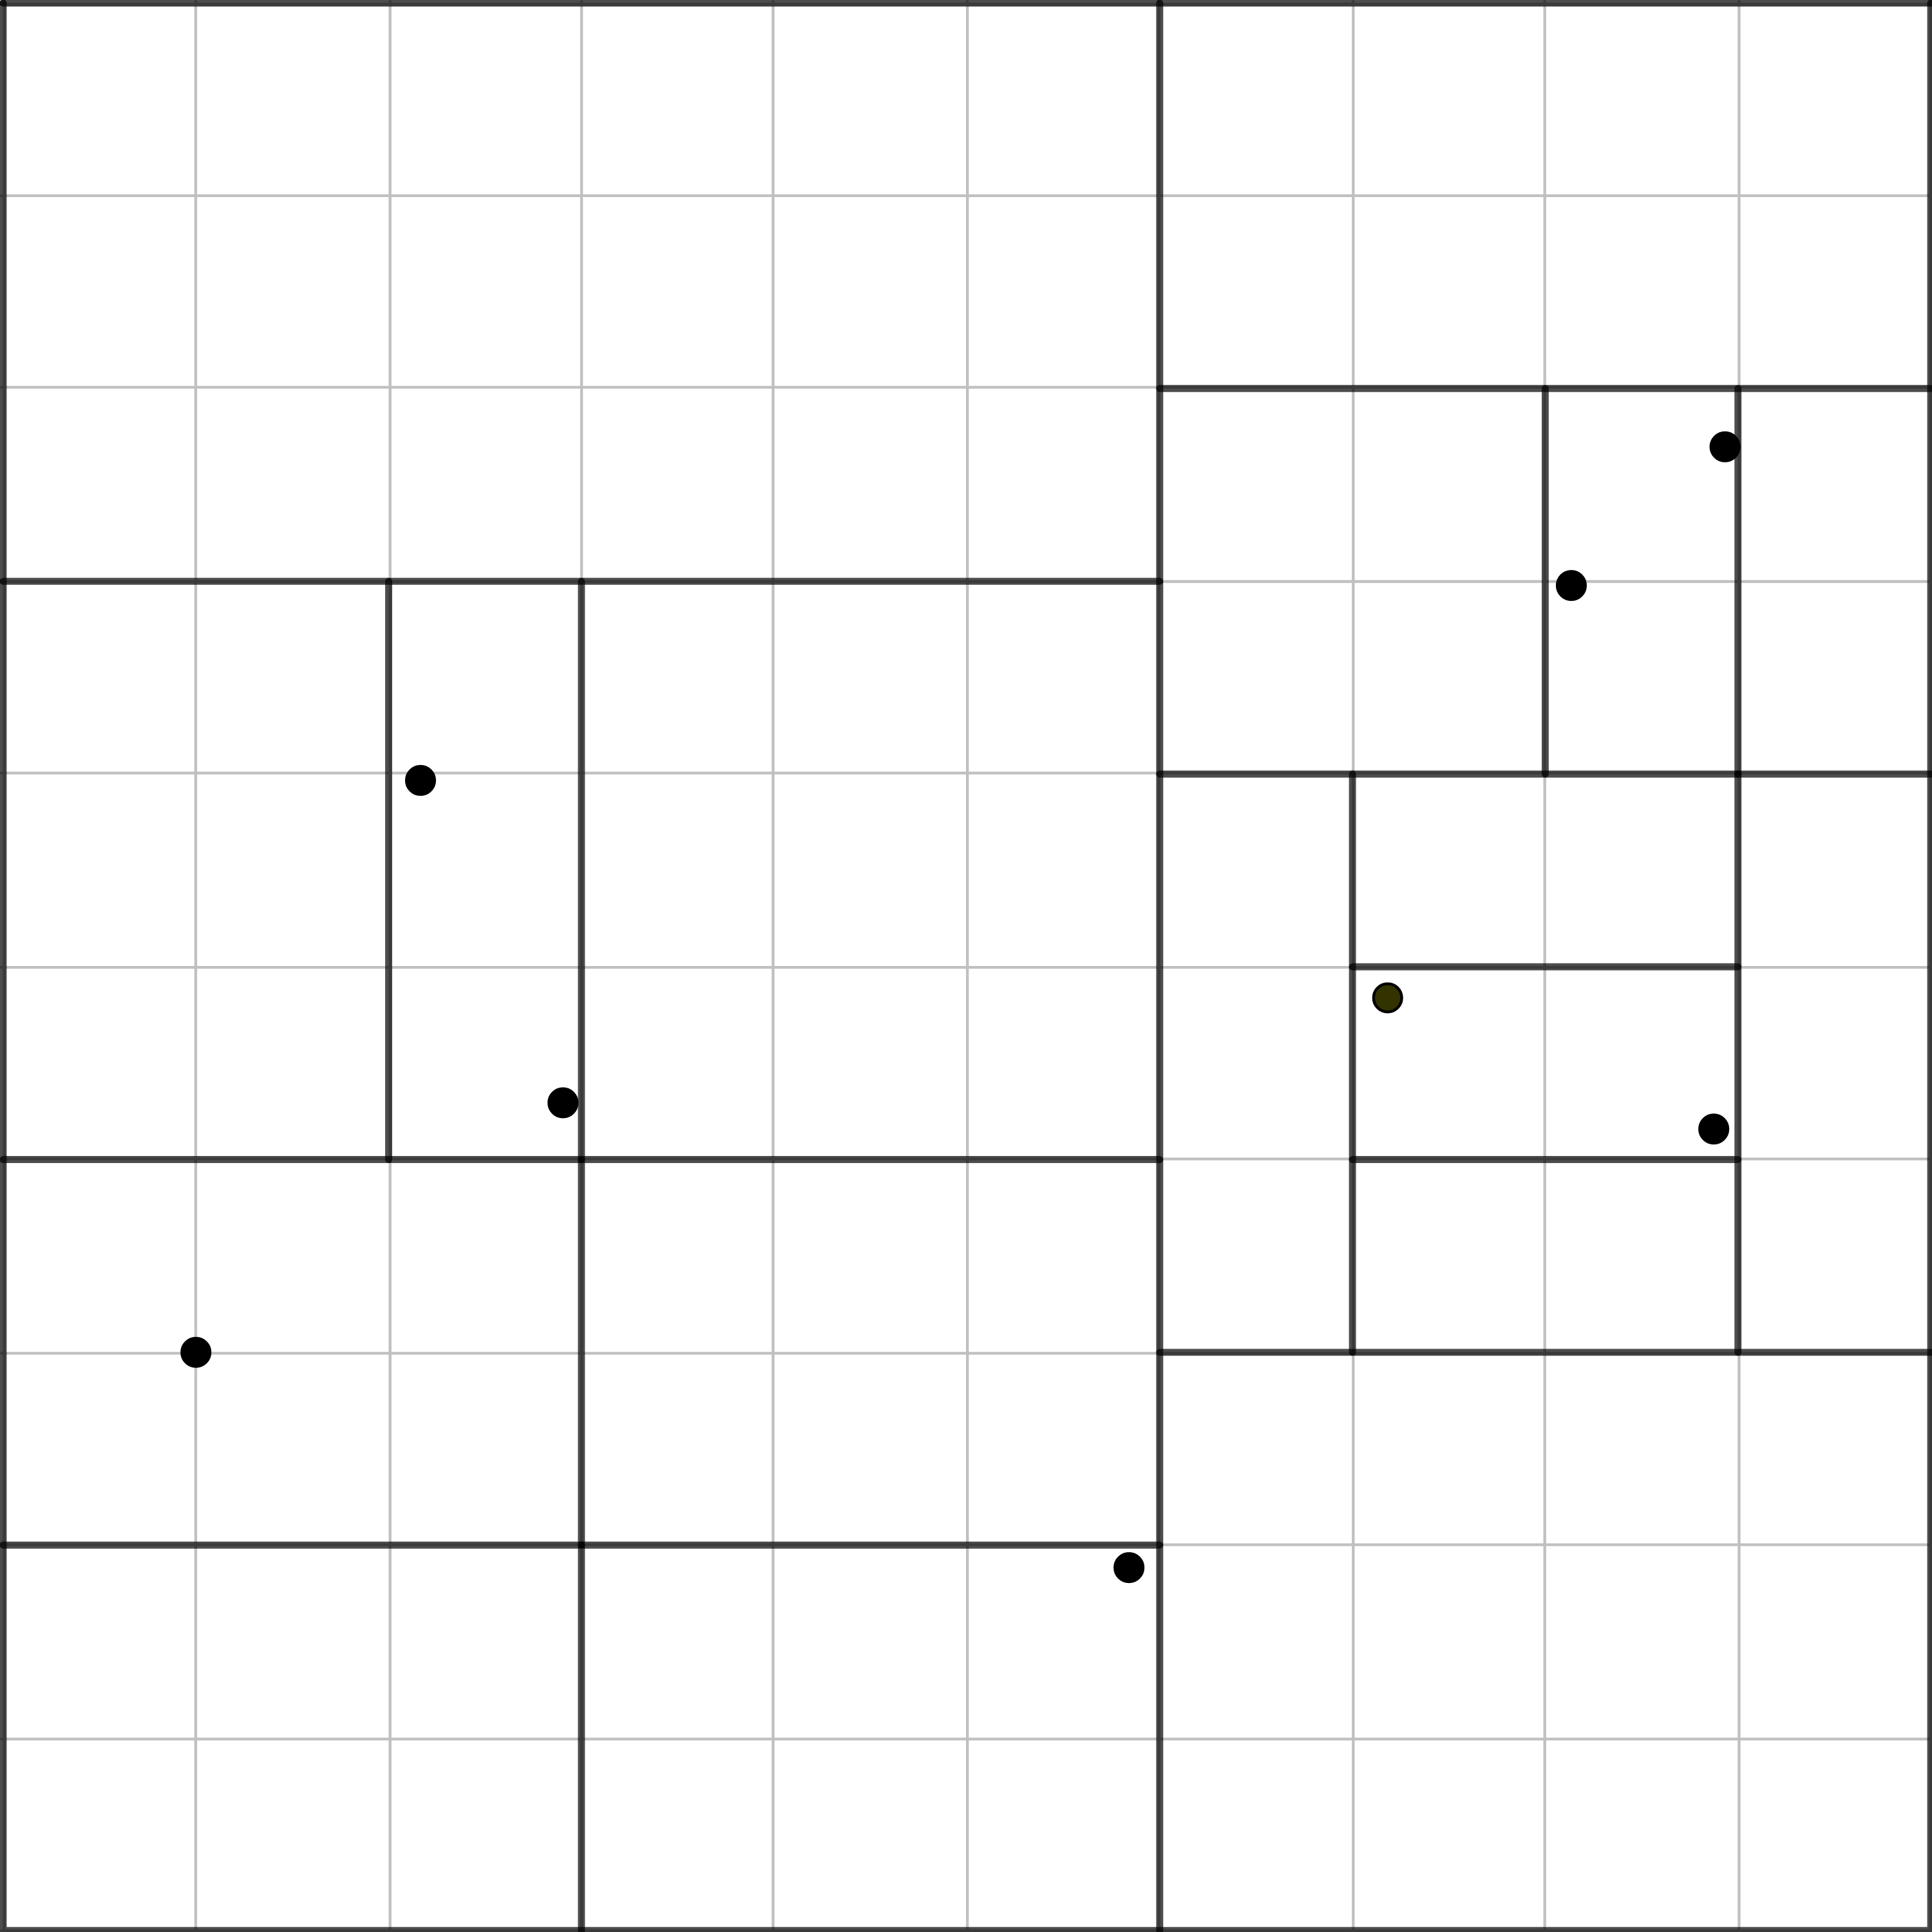
\includegraphics[width=0.7\textwidth]{images/20p2.png}
    \caption{AABB Hierarchy}
    \label{fig:20}
\end{figure}

\end{document}